\documentclass[a4paper]{article}
\usepackage{array, xcolor, lipsum, bibentry,fancyhdr}
\usepackage[scale=0.75,twoside,bindingoffset=5mm]{geometry}
\usepackage[onehalfspacing]{setspace}
\usepackage{amsmath, kotex, graphicx}
\usepackage{multirow}

\pagestyle{fancy}
\lhead{Drag Force Experiment}
\chead{}
\rhead{\thepage}
\renewcommand{\headrulewidth}{0.4pt}
%\renewcommand{\footrulewidth}{0.4pt}

\newcolumntype{P}[1]{>{\centering\arraybackslash}p{#1}}
\newcolumntype{M}[1]{>{\centering\arraybackslash}m{#1}}
\usepackage[utf8]{inputenc}
%\graphicspath{ {C:/Users/Sou/Pictures/images/} }

\title{Lab 6. Drag Force}
\author{16-087 이현동\quad 16-046 백승재\quad 16-078 이재문}
\date{April 14, 2017}

\begin{document}

\maketitle

\begin{abstract}
This experiment measures the position of the objects dropped to viscous liquid. Considering the effects of viscosity to the velocity at each time, we measured the position and velocity of the ball each moment. By analyzing this data, we could figure out the viscosity of the particular liquid.
\end{abstract}

\section{Introduction}
In this experiment, we will measure the terminal velocity of the ball in a viscous medium and determine the viscosity of the liquid. We will also introduce the idea of Stoke's law to determine the difference between the liquid with bounded area and non-bounded area.
% #################################################################
\section{Theory}
In this experiment, we are using a spherical object which experiences drag force by viscous fluid. When a spherical object is falling in a viscous fluid, the magnitude of drag force $f$ is almost directly proportional to the sphere's speed $v$. 
\begin{equation}
f = kv
\end{equation}
In this equation, $k$ is a constant which depends on the shape and size of the falling body. According to Stokes' law, this constant can be represented by $k = 6 \pi \eta r$ when $\eta$ is the viscosity of the liquid and $r$ is radius of the ball.\\ \\
Also, this experiment is conducted in a cylinder, which is a limited container. Since the object should 'penetrate' through the viscous liquid, the object experiences the wall effect. If we let the terminal velocity of the ball dropped in the unbounded medium $v_{T \infty}$ and in the bounded medium having inner diameter $D$ be $v_T$, the following equation holds between the variables.
\begin{equation}
\displaystyle \frac{v_T}{v_{T \infty}} = 1 - 2.014 \cdot \left(\frac{d}{D}\right)
\end{equation}

\section{Procedure}
\begin{enumerate}
\item{Calculate the density of the liquid by measuring the mass of specific volume of corn syrup. We used 20 ml of corn syrup to determine the density of it.}
\item{Measure the diameter and mass of 5 different balls to use in the experiment.}
\item{Drop the ball into the corn syrup and measure the time interval of the ball to drop one unit written on the mass cylinder.}
\item{Determine the viscosity of the liquid $\eta$. Wall effect should be also considered in this step to adjust the viscosity.}
\end{enumerate}

% #################################################################
\section{Results and Analysis}
First, we calculated the mass of corn syrup that we used. Measurement showed 26.6 g when we used 20 ml of corn syrup. This shows that the density of corn syrup $\rho_c$ is about 1.33 g/ml. \\ \newline
We used 5 different balls in this experiment. The configuration of each ball is shown in the following table.

% #################################################################
\begin{table}[htbp]
\begin{center}
\begin{tabular}{|c|c|c|c|c|c|}
\hline
 & $m_1$ & $m_2$ & $m_3$ & $m_4$ & $m_5$ \\ \hline 
Mass (g) & 0.03 & 0.11 & 0.26 & 0.52 & 0.89 \\ \hline
Diameter (mm) & 2 & 3 & 4 & 5 & 6\\ \hline
\end{tabular}
\caption{Mass and Diameter of the balls}
\end{center}
\end{table}
We conducted an experiment and measured the time elapsed for the ball to fall one unit in the mass cylinder, 10 ml. In the mass cylinder that we used, 10 ml had a vertical length about 1.625 cm.


% #################################################################
\section{Discussion}
We do the experiment for 2 to 6mm balls, and we can get almost same viscosity. But the viscosity goes high when the size of the ball goes big. \newline


\textbf{Source of Error}
\begin{itemize}
    \item{The speed of the ball can be changed by the position of the ball. We should place the ball in the center of the cylinder, but we cannot be perfect. }
    \item{The bubbles in the cylinder can affect to the speed. We just pour it in the cylinder, so there could be bubbles.}
\end{itemize}
In conclusion, we did the experiment which is measuring the drag force of the liquid, and we can check the viscosity of the liquid.
\begin{figure}[htbp]
    \begin{center}
    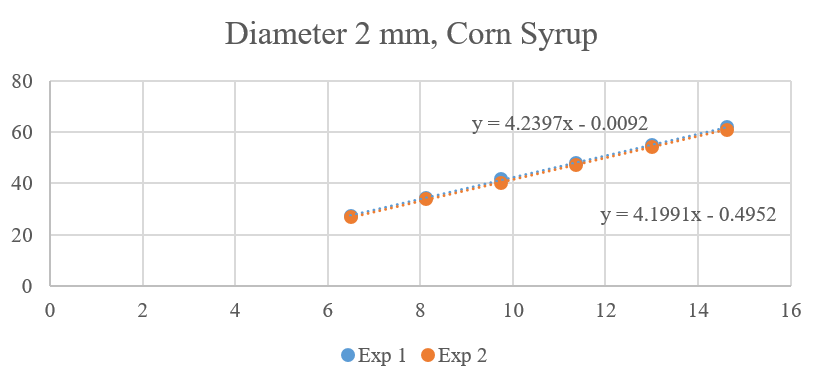
\includegraphics[scale=1]{exp1}
    \caption{Diameter 2 mm}
    \label{fig:my_label}
    \end{center}
\end{figure}

\end{document}
